% arara: xelatex: { shell: yes }
% arara: biber
% arara: nomencl
% arara: xelatex: { shell: yes }
% arara: xelatex: { shell: yes }
\documentclass[nolibertine, ngerman, algorithm, nomencl, minted]{ttlab-qualify}
% mögliche Optionen:
% - ngerman
% - english
% - minted
% - algorithm
% - nomencl
% - nolibertine
\usepackage{libertine}
\usepackage{biblatex}
\usepackage{listings}
%\usepackage{natbib}
\usepackage{hyperref}
\hypersetup{
    colorlinks=true,      % Aktiviert farbige Links
    urlcolor=blue,        % URLs in Blau
    linkcolor=black,      % Interne Links (z.B. Abschnittsverweise) in Schwarz
    citecolor=black,      % Zitatverweise (Bibliographie) in Schwarz
    filecolor=black,      % Dateilinks in Schwarz
    menucolor=black       % Acrobat-Menülinks in Schwarz
}
\urlstyle{same}

\addbibresource{bib.bib}

\begin{document}

\titlehead{
  Kenan Khauto\\
  7592047\\
  B.Sc Informatik\\
  Studienfachkombination / Schwerpunkt \\
  6\\
  kenan.khauto@stud.uni-frankfurt.de 
}
\subject{Seminararbeit Text Analytics}
\author{Kenan Khauto}
\title{Image Understanding}
\subtitle{Lernen visueller Konzepte beim Inferieren ohne finetuning}
\date{Abgabedatum: <Datum>}
\publishers{Goethe-Universität Frankfurt am Main\\Prof. Alexander Mehler}

\maketitle


\tableofcontents

\chapter{Einleitung}
Im Bereich der künstlichen Intelligenz und des maschinellen Lernens hat sich in den letzten Jahren eine bemerkenswerte Entwicklung 
vollzogen, insbesondere im Verständnis visueller Konzepte durch Modelle wie CLIP (Contrastive Language–Image Pretraining). 
Diese Modelle haben das traditionelle Paradigma, das umfangreiche Fine-Tuning und spezialisierte Datensätze erforderte, herausgefordert 
und bieten neue Wege, wie Maschinen Bilder und Texte in einem zusammenhängenden Rahmen verstehen können.


Die Kernfrage, die wir in diesem Seminar untersuchen, lautet: "Wie können KI-Modelle wie CLIP visuelle Konzepte effektiv durch 
Inferenz verstehen und interpretieren, ohne dass ein umfangreiches Fine-Tuning erforderlich ist?" Diese Frage berührt die Grundlagen 
der Art und Weise, wie maschinelle Lernmodelle trainiert und angewendet werden, insbesondere im Kontext der Integration von visuellen und 
textuellen Daten.


CLIP, ein Produkt von OpenAI, repräsentiert einen Durchbruch in der Art und Weise, wie Maschinen lernen, Bilder und Texte zu verbinden. 
Anstatt sich auf umfangreiche, spezialisierte Datensätze zu verlassen, nutzt CLIP ein breites Spektrum an Internetdaten und lernt, 
visuelle Konzepte direkt aus einer Vielzahl von Bildern und den dazugehörigen Beschreibungen zu extrahieren. Dieser Ansatz ermöglicht 
es dem Modell, eine breite Palette von visuellen Konzepten zu verstehen, ohne für jedes neue Konzept speziell angepasst zu werden.


In diesem Seminar werden wir die Mechanismen hinter CLIP und ähnlichen Modellen erforschen. Wir werden untersuchen, wie diese Modelle 
trainiert werden, ihre Fähigkeit, visuelle Daten zu interpretieren, und die Herausforderungen, denen sie gegenüberstehen, wie zum Beispiel 
die Behandlung von Verzerrungen und die Generalisierbarkeit ihrer Erkenntnisse. Darüber hinaus werden wir diskutieren, wie diese Technologien 
in verschiedenen Anwendungsfeldern eingesetzt werden könnten, von der automatisierten Bildbeschreibung bis hin zur Verbesserung 
der Mensch-Maschine-Interaktion.

\chapter{Hauptteil}
\section{Theoretischer Hintergrund}
Dieser Abschnitt stellt die theoretischen Grundlagen vor, die für das Verständnis der Funktionsweise von KI-Modellen wie CLIP (Contrastive Language–Image Pretraining) essentiell sind. Hier werden die Kernelemente des maschinellen Lernens, die Besonderheiten des Deep Learning und die Bedeutung des kontrastiven Lernens für die Verarbeitung von Bild- und Textdaten erörtert.

\subsection{Grundlagen des maschinellen Lernens}

Maschinelles Lernen ist ein Teilgebiet der künstlichen Intelligenz, das sich mit der Entwicklung von Algorithmen beschäftigt, die Computern das Lernen aus Daten ermöglichen. Die Hauptzielsetzung des maschinellen Lernens ist es, Muster in Daten zu erkennen und auf Basis dieser Muster Vorhersagen oder Entscheidungen zu treffen.

\textbf{Überwachtes vs. unüberwachtes Lernen:} Überwachtes Lernen bezieht sich auf Lernprozesse, bei denen das Modell anhand von Beispieldaten und bekannten Ausgabewerten trainiert wird. Unüberwachtes Lernen hingegen befasst sich mit dem Finden von Mustern oder Strukturen in Daten, ohne vorherige Kenntnis der Ausgabewerte.

\textbf{Verstärkendes Lernen:} Eine weitere wichtige Lernmethode ist das verstärkende Lernen, bei dem ein Modell durch Belohnungen lernt, bestimmte Aktionen in einer Umgebung auszuführen, um ein bestimmtes Ziel zu erreichen.

\subsection{Deep Learning und neuronale Netzwerke}

Deep Learning, eine Unterklasse des maschinellen Lernens, basiert auf künstlichen neuronalen Netzwerken mit vielen Schichten (sogenannten "tiefen" Netzwerken). Diese Netzwerke sind in der Lage, komplexe Muster in großen Datenmengen zu erkennen.

\begin{figure}[h]
	\centering
	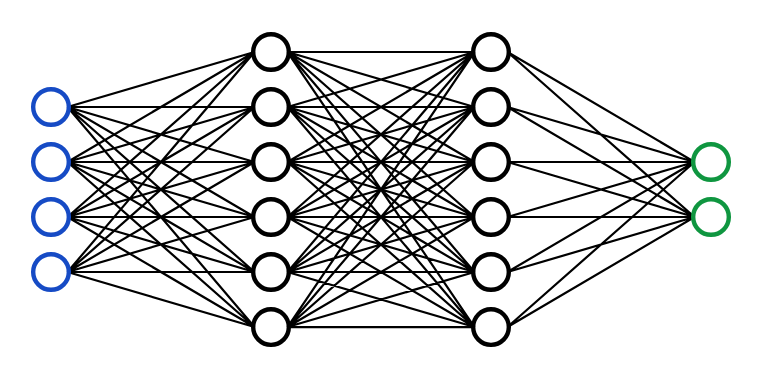
\includegraphics[scale=0.4]{static/FCnetwork.png}
	\caption{A simple fully connected neural network, see \url{https://victorzhou.com/series/neural-networks-from-scratch/}}
	\label{fig:2.1}
\end{figure}

\textbf{Convolutional Neural Networks (CNNs):} Speziell für die Bildverarbeitung sind CNNs von entscheidender Bedeutung. Sie sind darauf ausgelegt, hierarchische Muster in Bildern zu erkennen, was sie ideal für Aufgaben wie Bildklassifikation und Objekterkennung macht.
\begin{figure}[h]
	\centering
	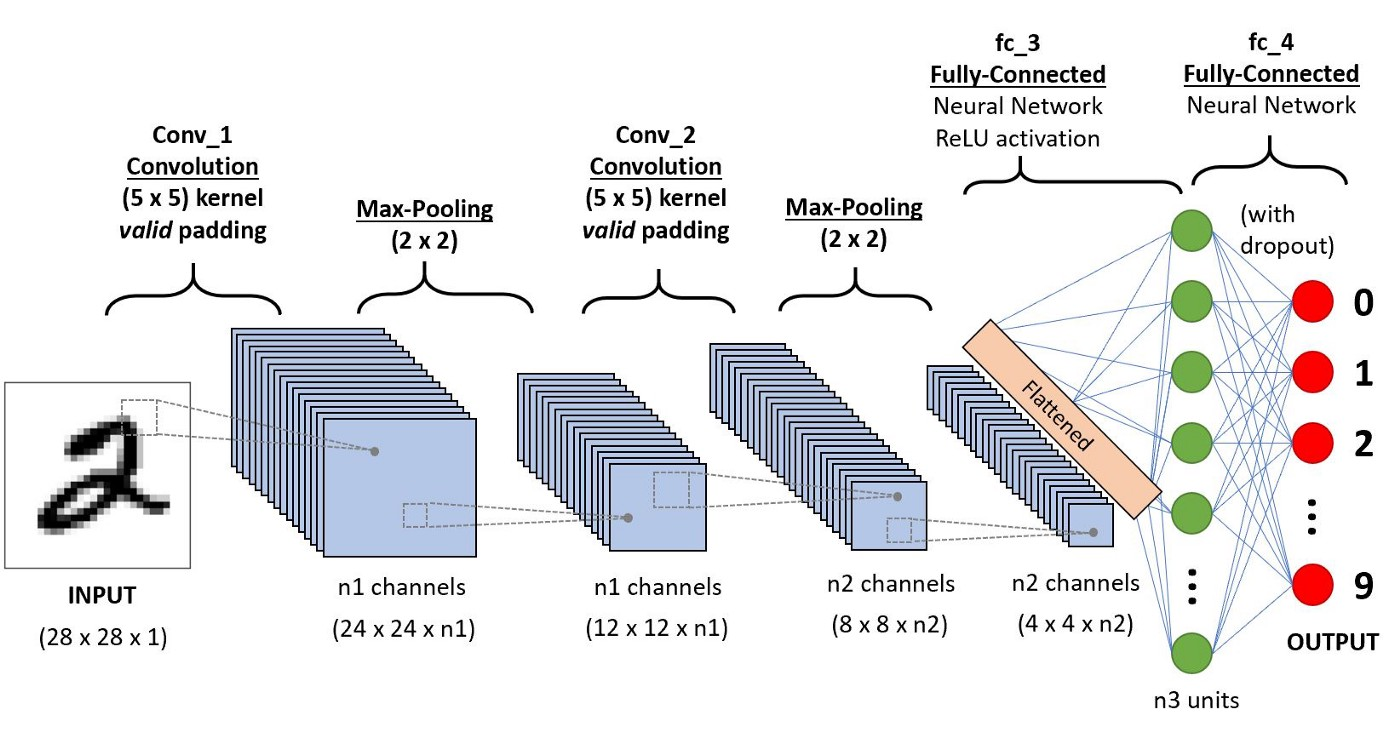
\includegraphics[scale=0.2]{static/cnn.jpeg}
	\caption{Convolutional neural network (CNN), see \url{https://paperswithcode.com/methods/category/convolutional-neural-networks}}
	\label{fig:2.2}
\end{figure}

\textbf{Transformer-Modelle:} Ursprünglich in der Verarbeitung natürlicher Sprache eingesetzt, haben Transformer-Modelle aufgrund ihrer Fähigkeit, langfristige Abhängigkeiten in Daten zu erkennen, zunehmend Anwendung in anderen Bereichen, einschließlich der Bildverarbeitung, gefunden.
\begin{figure}[h]
	\centering
	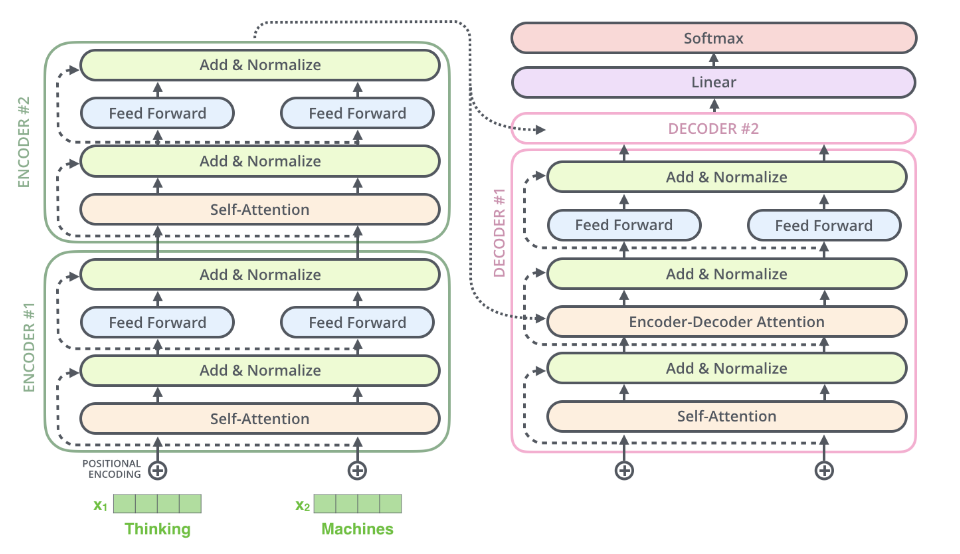
\includegraphics[scale=0.5]{static/transformer.png}
	\caption{Transformer with two encoders, 2 decoders and a fully connected layer for prediction, see \url{http://jalammar.github.io/illustrated-transformer/}}
	\label{fig:2.3}
\end{figure}

\subsection{Kontrastives Lernen und CLIP}
Kontrastives Lernen ist eine Technik, die darauf abzielt, ähnliche Datenpunkte näher zusammenzubringen und unähnliche weiter voneinander zu entfernen. CLIP verwendet kontrastives Lernen, um die Beziehungen zwischen Bildern und Text zu verstehen.

\textbf{Funktionsweise von CLIP:} CLIP wird mit einer Vielzahl von Bildern und den dazugehörigen Textbeschreibungen trainiert. Das Modell lernt, die Verbindungen zwischen Bildern und Texten zu verstehen, was es ihm ermöglicht, eine breite Palette von Bildinhalten effektiv zu interpretieren.

\textbf{Vorteile gegenüber traditionellen Ansätzen:} Im Gegensatz zu traditionellen Bilderkennungsmodellen, die oft umfangreiches Fine-Tuning für spezifische Aufgaben benötigen, kann CLIP vielfältige visuelle Konzepte anhand seiner Trainingsdaten erkennen und interpretieren, was eine größere Flexibilität und Anpassungsfähigkeit bedeutet.
\section{Analyse von CLIP}
CLIP ist ein neuronales Netzwerk, das anhand einer Vielzahl von Bildern und den zugehörigen Textbeschreibungen trainiert wurde. Dieses Training ermöglicht es ihm, sowohl visuelle als auch textuelle Eingaben zu verstehen und zu interpretieren. Im Gegensatz zu traditionellen Modellen, die eine aufgabenspezifische Feinabstimmung erfordern, ist CLIP für eine breite Palette visueller Aufgaben direkt einsetzbar.

\subsection{Architektur}
Das Modell besteht aus zwei Hauptkomponenten: einem Text-Encoder und einem Bild-Encoder. Der Text-Encoder verarbeitet textuelle Eingaben, während der Bild-Encoder sich um visuelle Eingaben kümmert. Beide Encoder wandeln ihre jeweiligen Eingaben in einen gemeinsamen Einbettungsraum um, was dem Modell ermöglicht, die beiden unterschiedlichen Datentypen direkt zu vergleichen und zu verknüpfen.
\begin{figure}[h]
	\centering
	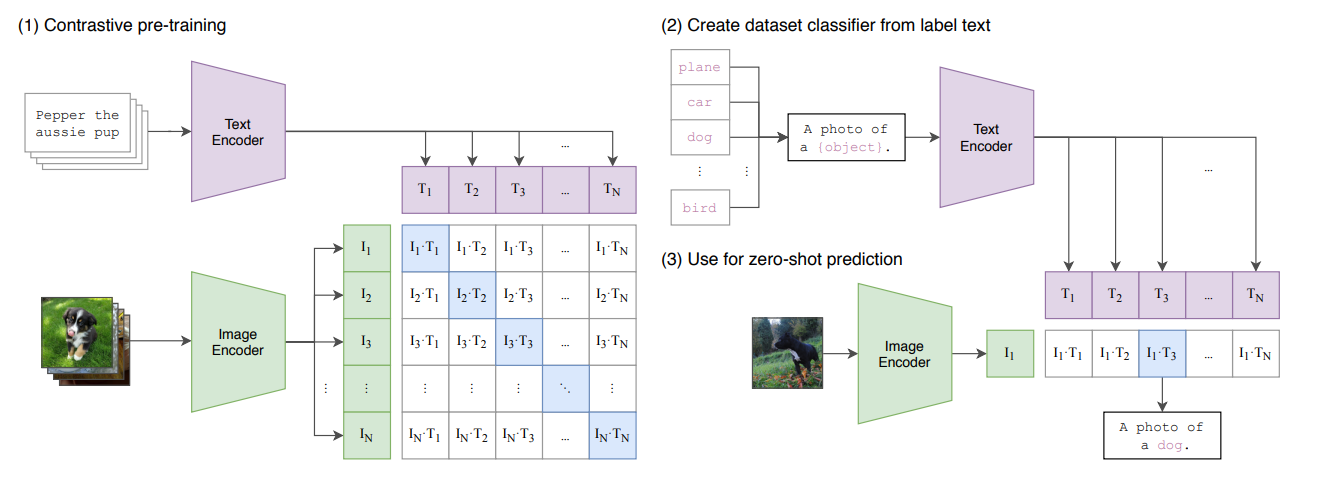
\includegraphics[scale=0.4]{static/CLIP.png}
	\caption{CLIP, Bild von (\cite{radford2021learning})}
	\label{fig:2.4}
\end{figure}
\subsubsection{Text-Encoder}
Der Text-Encoder in CLIP basiert auf einer Transformer-Architektur. Jedes Wort im Text wird in eine Vektordarstellung umgewandelt. Der Transformer verwendet Selbst-Attention, um die Bedeutung jedes Wortes im Kontext des gesamten Textes zu verstehen. Ziel des Text-Encoders ist es, eine Darstellung des Textes zu erzeugen, die dessen semantischen Inhalt in Bezug auf mögliche Bildinhalte widerspiegelt.

\subsubsection{Bild-Encoder}
Der Bild-Encoder in CLIP ist nicht ausschließlich auf Convolutional Neural Networks (CNNs) beschränkt, sondern kann auch Vision Transformers (ViTs) umfassen. Die Wahl des spezifischen Netzwerktyps hängt von der gewünschten Leistung und den Eigenschaften der Aufgabe ab:
\begin{itemize}
    \item \textbf{CNN-basierte Encoder}: Traditionelle CNN-Architekturen sind effektiv in der Erkennung lokaler Muster und Texturen in Bildern. Sie wandeln das Bild in eine Serie von Vektorrepräsentationen um, die die visuellen Inhalte des Bildes kodieren.
    \item \textbf{Vision Transformers}: ViTs nähern sich der Bildverarbeitung auf eine andere Weise an, indem sie das Bild in eine Sequenz von Patches zerlegen und diese Patches ähnlich wie Wörter in einem Satz behandeln. Dies ermöglicht es ViTs, sowohl lokale als auch globale Kontextinformationen aus dem Bild zu erfassen.
\end{itemize}
Der Hauptzweck des Bild-Encoders, unabhängig von der gewählten Architektur, besteht darin, 
eine Darstellung des Bildes zu erzeugen, die in demselben Vektorraum wie der Text-Encoder liegt, 
um eine direkte Vergleichbarkeit und Verknüpfung von Text und Bild zu ermöglichen.

Für Leser, die sich tiefergehend mit der Theorie und Anwendung von Transformern beschäftigen möchten, 
empfehle ich die grundlegenden Papers (\cite{vaswani2017attention}) und (\cite{dosovitskiy2020image}).
Diese zwei Werke bieten eine umfassende Einführung in das Konzept der Transformer und ViTs und legt 
den Grundstein für viele moderne Ansätze in der Verarbeitung natürlicher Sprache und Bilderkennung.

\subsection{Integration und gemeinsamer Einbettungsraum}
Die zentrale Innovation von CLIP besteht darin, dass beide Encoder - der Text- und der Bild-Encoder - darauf trainiert sind, ihre Ausgaben in einem gemeinsamen Einbettungsraum zu repräsentieren. Dies ermöglicht es dem Modell, die Beziehung zwischen Texten und Bildern effektiv zu verstehen und auf dieser Basis präzise Entscheidungen zu treffen.

\begin{itemize}
	\item \textbf{\textit{Vektorraumbildung: }} CLIP lernt, Bilder und Texte in einen hochdimensionalen Vektorraum zu transformieren. Dabei werden Bild- und Textrepräsentationen so angepasst, dass korrespondierende Paare nahe beieinander liegen.
	\item \textbf{\textit{Kontrastives Lernen: }}Das Modell verwendet einen kontrastiven Lernansatz, um die Distanz zwischen übereinstimmenden Bild-Text-Paaren zu minimieren und die Distanz zwischen nicht übereinstimmenden Paaren zu maximieren. Dieses Training fördert eine effektive Abbildung beider Modalitäten in den gemeinsamen Raum.
\end{itemize}

\subsection{Kontrastives Lernen im Detail}
Der kontrastive Lernansatz von CLIP basiert darauf, dass das Modell
lernt, korrespondierende Text-Bild-Paare miteinander zu verknüpfen,
während es gleichzeitig nicht passende Paare unterscheidet. Dieser
Ansatz erlaubt es dem Modell, eine umfassende und nuancierte Sicht
auf die Beziehungen zwischen Texten und Bildern zu entwickeln, was für die 
Zero-Shot-Lernfähigkeiten von CLIP entscheidend ist.


\subsubsection{Vektoreinbettungen}
Sei \( \textbf{I} \) ein Bild und \( \textbf{T} \) ein Text, dann werden die Einbettungen durch die Encoder-Funktionen wie folgt generiert:
\begin{align*}
\text{Bild-Einbettung:} \quad & \textbf{v}_I = f_{\text{Bild}}(\textbf{I}) \\
\text{Text-Einbettung:} \quad & \textbf{v}_T = f_{\text{Text}}(\textbf{T})
\end{align*}
wobei \( f_{\text{Bild}} \) und \( f_{\text{Text}} \) die Funktionen des Bild- bzw. Text-Encoders sind.

\subsubsection{Ähnlichkeitsberechnung}
Die Ähnlichkeit zwischen einem Bild- und einem Textvektor wird durch das Skalarprodukt ihrer normalisierten Vektoren berechnet:
\begin{align*}
\text{sim}(\textbf{I}, \textbf{T}) = \frac{\textbf{v}_I \cdot \textbf{v}_T}{\| \textbf{v}_I \| \, \| \textbf{v}_T \|}
\end{align*}

Das kann man in \ref{fig:2.4} sehen.
\subsubsection{Training und kontrastiver Verlust}
Das Training von CLIP erfolgt durch Minimierung des kontrastiven Verlustes. Für ein Batch von \( N \) Bild-Text-Paaren wird der Verlust für ein Paar \( (i, j) \) berechnet als:
\begin{align*}
L_{i,j} = -\log \frac{\exp(\text{sim}(\textbf{v}_{I_i}, \textbf{v}_{T_j}) / \tau)}{\sum_{k=1}^{N} \exp(\text{sim}(\textbf{v}_{I_i}, \textbf{v}_{T_k}) / \tau)}
\end{align*}
Hierbei ist:
\begin{itemize}
 \item \( \tau \) ein Temperaturparameter ist, der die Schärfe der Wahrscheinlichkeitsverteilung beeinflusst,
 \item \(\textbf{v}_{T_k}\)die Embedings der negativen Beispiele (nicht korrespondierende Bilder),
\end{itemize}

Diese Formel zielt darauf ab, die Wahrscheinlichkeit zu maximieren, dass das korrekte Bild-Text-Paar unter Berücksichtigung aller anderen Paare im Batch als das ähnlichste Paar ausgewählt wird. Der Logarithmus im Zähler bewirkt, dass das korrekte Paar einen hohen Beitrag zum Gesamtverlust leistet, wenn es nicht als ähnlichstes Paar identifiziert wird. Im Nenner summiert sich der Beitrag aller Paare im Batch, was die Unterscheidung zwischen korrekten und inkorrekten Paaren fördert.

\subsection{Zero-Shot Learning in CLIP}
\subsubsection{Konzept}
Zero-Shot Learning bezieht sich auf die Fähigkeit des Modells,
Aufgaben zu verstehen und durchzuführen, für die es nicht 
explizit trainiert wurde. Im Kontext von CLIP bedeutet dies, 
Bilder und Konzepte zu erkennen und zu interpretieren, 
die es während des Trainings nie gesehen hat.

\subsubsection{Mechanismus}
Dies wird durch das generalisierte Verständnis des Modells von Bildern und Texten 
erreicht. Durch das Training mit einem vielfältigen Datensatz lernt CLIP eine breite 
Palette von visuellen Stilen, Objekten und Konzepten, was ihm eine gute Generalisierung 
auf neue, ungesehene Aufgaben ermöglicht.

\subsubsection{Anwendungen}
Diese Eigenschaft macht CLIP außerordentlich vielseitig. Es kann für verschiedene 
Aufgaben wie Objekterkennung, Inhaltsmoderation und sogar kreative Anwendungen wie 
das Generieren von Bildern aus Textbeschreibungen verwendet werden.

\begin{minted}[frame=lines, framesep=2mm, baselinestretch=1.2, fontsize=\footnotesize]{python}
model_id = "openai/clip-vit-base-patch32"
processor = CLIPProcessor.from_pretrained(model_id)
model = CLIPModel.from_pretrained(model_id)

image = read_image(image_name="2.jpg")
image = np.expand_dims(image, axis=0)

labels = ["A photo of a piano", 
"Someone playing the piano", 
"A photo of a guitar", 
"A photo of a piano in a white background",
"A very big dog eating hotdogs", 
"A fluffy cat", 
"A photo of the earth from the dark space"]

labels = processor(
text=labels,
images=None,
padding=True,
return_tensors="pt"
).to(device)

text_emb = model.get_text_features(**labels)
text_emb = text_emb.detach().cpu().numpy()
text_emb = text_emb / np.linalg.norm(text_emb, axis=0)

image = processor(
text=None,
images=image,
return_tensors="pt"
)["pixel_values"].to(device)

image_emb = model.get_image_features(image)
image_emb = image_emb.detach().cpu().numpy()

similarities = np.dot(image_emb, text_emb.T)

index = np.argmax(similarities, axis=1).item()

result = labesl[index]
\end{minted}

Im obigen Codestück sieht man grob, wie man CLIP für image Classification ohne fine-tuning nutzen kann.
Der komplette Code findet man auf \url{https://github.com/KenanKhauto/zero-shot-learning}.
Die Labels habe ich selber manuell erstellt.
Und das Bild, was ich als Eingabe benutzt habe, ist ein Klavier mit einem weißen Hintergrund. Und die Ausgabe des Models ist auch diese Beschreibung.
Das zeigt vorallem, dass das Model nicht nur Objekte klassifiziert, sondern auch das komplette Bild versteht.
Das war ein einfaches Beispiel über Image Classification. Wir werden aber im Section-\ref{sec:Fallstudien-Anwendung} 
noch ein detailiertes Bespiel sehen, wie man Object Localization und Object Detection mithilfe von 
CLIP machen kann.
\subsection{Vergleichsanalyse}

\subsubsection{Traditionelle Vision-Modelle}
Frühere Modelle in der Computer Vision waren in der Regel aufgabenspezifisch (z.B. Modelle zur Objekterkennung, Bildsegmentierung) und erforderten umfangreiche Feinabstimmungen mit beschrifteten Daten für jede Aufgabe.

\subsubsection{Multimodale Modelle}
Andere zeitgenössische Modelle wie Googles BERT und OpenAIs GPT-3 haben fortgeschrittene 
Fähigkeiten in ihren jeweiligen Bereichen (Text- und Sprachverarbeitung), sind jedoch nicht 
inhärent darauf ausgelegt, die Beziehung zwischen Text und Bildern zu verstehen, 
wie es bei CLIP der Fall ist.

\subsubsection{Vorteile von CLIP}
CLIPs Fähigkeit, textuelle und visuelle Informationen zu verstehen und zu verknüpfen, 
ohne aufgabenspezifisches Training, hebt es ab. Seine Fähigkeiten zum Zero-Shot Learning 
reduzieren deutlich den Bedarf an großen annotierten Datensätzen für neue Aufgaben.

\section{Fallstudien / Anwendungen}
\label{sec:Fallstudien-Anwendung}
Hier erwähnen wo und wie CLIP in image understanding paper benutzt wurde.
\section{Diskussion von Herausforderungen und Grenzen}
\section{Zukünftige Richtungen und mögliche Verbesserungen}
Füge Attention is all you need und Vits papers als Quellen fürs Verstehen, wie Transformer genau funktionieren.
\printbibliography
\appendix
\chapter{Anhang 1}
	\begin{minted}{python}
		import torch
		import torchvision
		import torchvision.transforms as transforms
		from transformers import CLIPProcessor, CLIPModel
		import matplotlib.pyplot as plt
		from torch.utils.data import DataLoader
		from datasets import load_dataset
		import numpy as np
		
		imagenette = load_dataset(
			"frgfm/imagenette",
			"320px",
			split="validation",
			revision="4d512db"
		)
		
		labels = imagenette.info.features["label"].names
		clip_labels = [f"A photo of {x}" for x in labels]
		clip_labels
	\end{minted}

\end{document}
